\documentclass{article}
\usepackage{amsmath}
\usepackage[mathletters]{ucs}
\usepackage[utf8x]{inputenc}
\usepackage[margin=1.5in]{geometry}
\usepackage{enumerate}
\newtheorem{theorem}{Theorem}
\usepackage[dvipsnames]{xcolor}
\usepackage{pgfplots}
\setlength{\parindent}{0cm}
\usepackage{graphics}
\usepackage{graphicx} % Required for including images
\usepackage{subcaption}
\usepackage{bigintcalc}
\usepackage{pythonhighlight} %for pythonkode \begin{python}   \end{python}
\usepackage{appendix}
\usepackage{arydshln}
\usepackage{physics}
\usepackage{tikz-cd}
\usepackage{booktabs} 
\usepackage{adjustbox}
\usepackage{mdframed}
\usepackage{relsize}
\usepackage{physics}
\usepackage[thinc]{esdiff}
\usepackage{fixltx2e}
\usepackage{esint}  %for lukket-linje-integral
\usepackage{xfrac} %for sfrac
\usepackage{hyperref} %for linker, må ha med hypersetup
\usepackage[noabbrev, nameinlink]{cleveref} % to be loaded after hyperref
\usepackage{amssymb} %\mathbb{R} for reelle tall, \mathcal{B} for "matte"-font
\usepackage{listings} %for kode/lstlisting
\usepackage{verbatim}
\usepackage{xcolor}
\usepackage{graphicx,wrapfig,lipsum,caption} %for wrapping av bilder
\usepackage{mathtools} %for \abs{x}
\usepackage[norsk]{babel}
\definecolor{codegreen}{rgb}{0,0.6,0}
\definecolor{codegray}{rgb}{0.5,0.5,0.5}
\definecolor{codepurple}{rgb}{0.58,0,0.82}
\definecolor{backcolour}{rgb}{0.95,0.95,0.92}

\lstdefinestyle{mystyle}{
    backgroundcolor=\color{backcolour},   
    commentstyle=\color{codegreen},
    keywordstyle=\color{magenta},
    numberstyle=\tiny\color{codegray},
    stringstyle=\color{codepurple},
    basicstyle=\ttfamily\footnotesize,
    breakatwhitespace=false,         
    breaklines=true,                 
    captionpos=b,                    
    keepspaces=true,                 
    numbers=left,                    
    numbersep=5pt,                  
    showspaces=false,                
    showstringspaces=false,
    showtabs=false,                  
    tabsize=2
}

\lstset{style=mystyle}
\author{Oskar Idland}
\title{FYS-1120 Oblig 1}
\date{}
\begin{document}
\maketitle
\newpage

\section*{a)}
  Ettersom en partikkel i origo vil oppleve like krefter fra alle retninger vil netto feltet være lik null. 
  Uten noen annen informasjon vet vi at potensialet er konstant. 

\section*{b)}
  Vi ser på én av linjene først og bruker superposisjon for å finne potensialet av alle linjene. Vi bruker linjen som ligger fremst på x-aksen med endepunkter i $ (a,-a,0) $ og $ (a,a,0) $. 
  \[
  V(\mathbf{z}) = ∫ _C \frac{\rho _l \mathrm{d}l}{4 \pi ϵ_0 R}
  \]
  \[
  V(\mathbf{z}) = ∫ _C \frac{Q}{32 a\pi ϵ_{0}R}
  \]
  \[
  \mathbf{R} = \mathbf{r} - \mathbf{r}' = (0,0,z) - (a,y,0) = (-a,-y,z)
  \]
  \[
  V(\mathbf{z}) = ∫ _{-a} ^{a} \frac{Q}{32 a π ϵ_{0} \sqrt{a^{2} + y^{2} + z^{2}} } \mathrm{d}y
  \]
  \[
  C = \sqrt{a^2 + z^2} 
  \]
  \[
  V(\mathbf{z}) = ∫ _{-a} ^{a} \frac{Q}{32a \pi ϵ_{0} \sqrt{C^{2} + y^{2}} } \mathrm{d}y
  \]
  \[
  V(\mathbf{z}) = \frac{Q}{32a \pi ϵ_0} \bigg[ \operatorname{arcsinh} \frac{y}{C} \bigg]_{-a}^{a} = \frac{Q}{16 a \pi ϵ_0} \operatorname{arcsinh} \left(\frac{a}{\sqrt{a^2 + z^2}}\right)_{}^{}
  \]
  Nå har vi funnet potensialet fra én av linjene. Ganger vi med fire får vi potesnialet fra alle. 
  \begin{equation} \label{Electric Potential 4lines }
    V(\mathbf{z}) = \frac{Q}{4a \pi ϵ_0} \operatorname{arcsinh} \left( \frac{a}{\sqrt{a^{2} + z^{2}}} \right) 
  \end{equation}
\newpage
\section*{c)}
  \begin{figure}[h!]
    \centering
    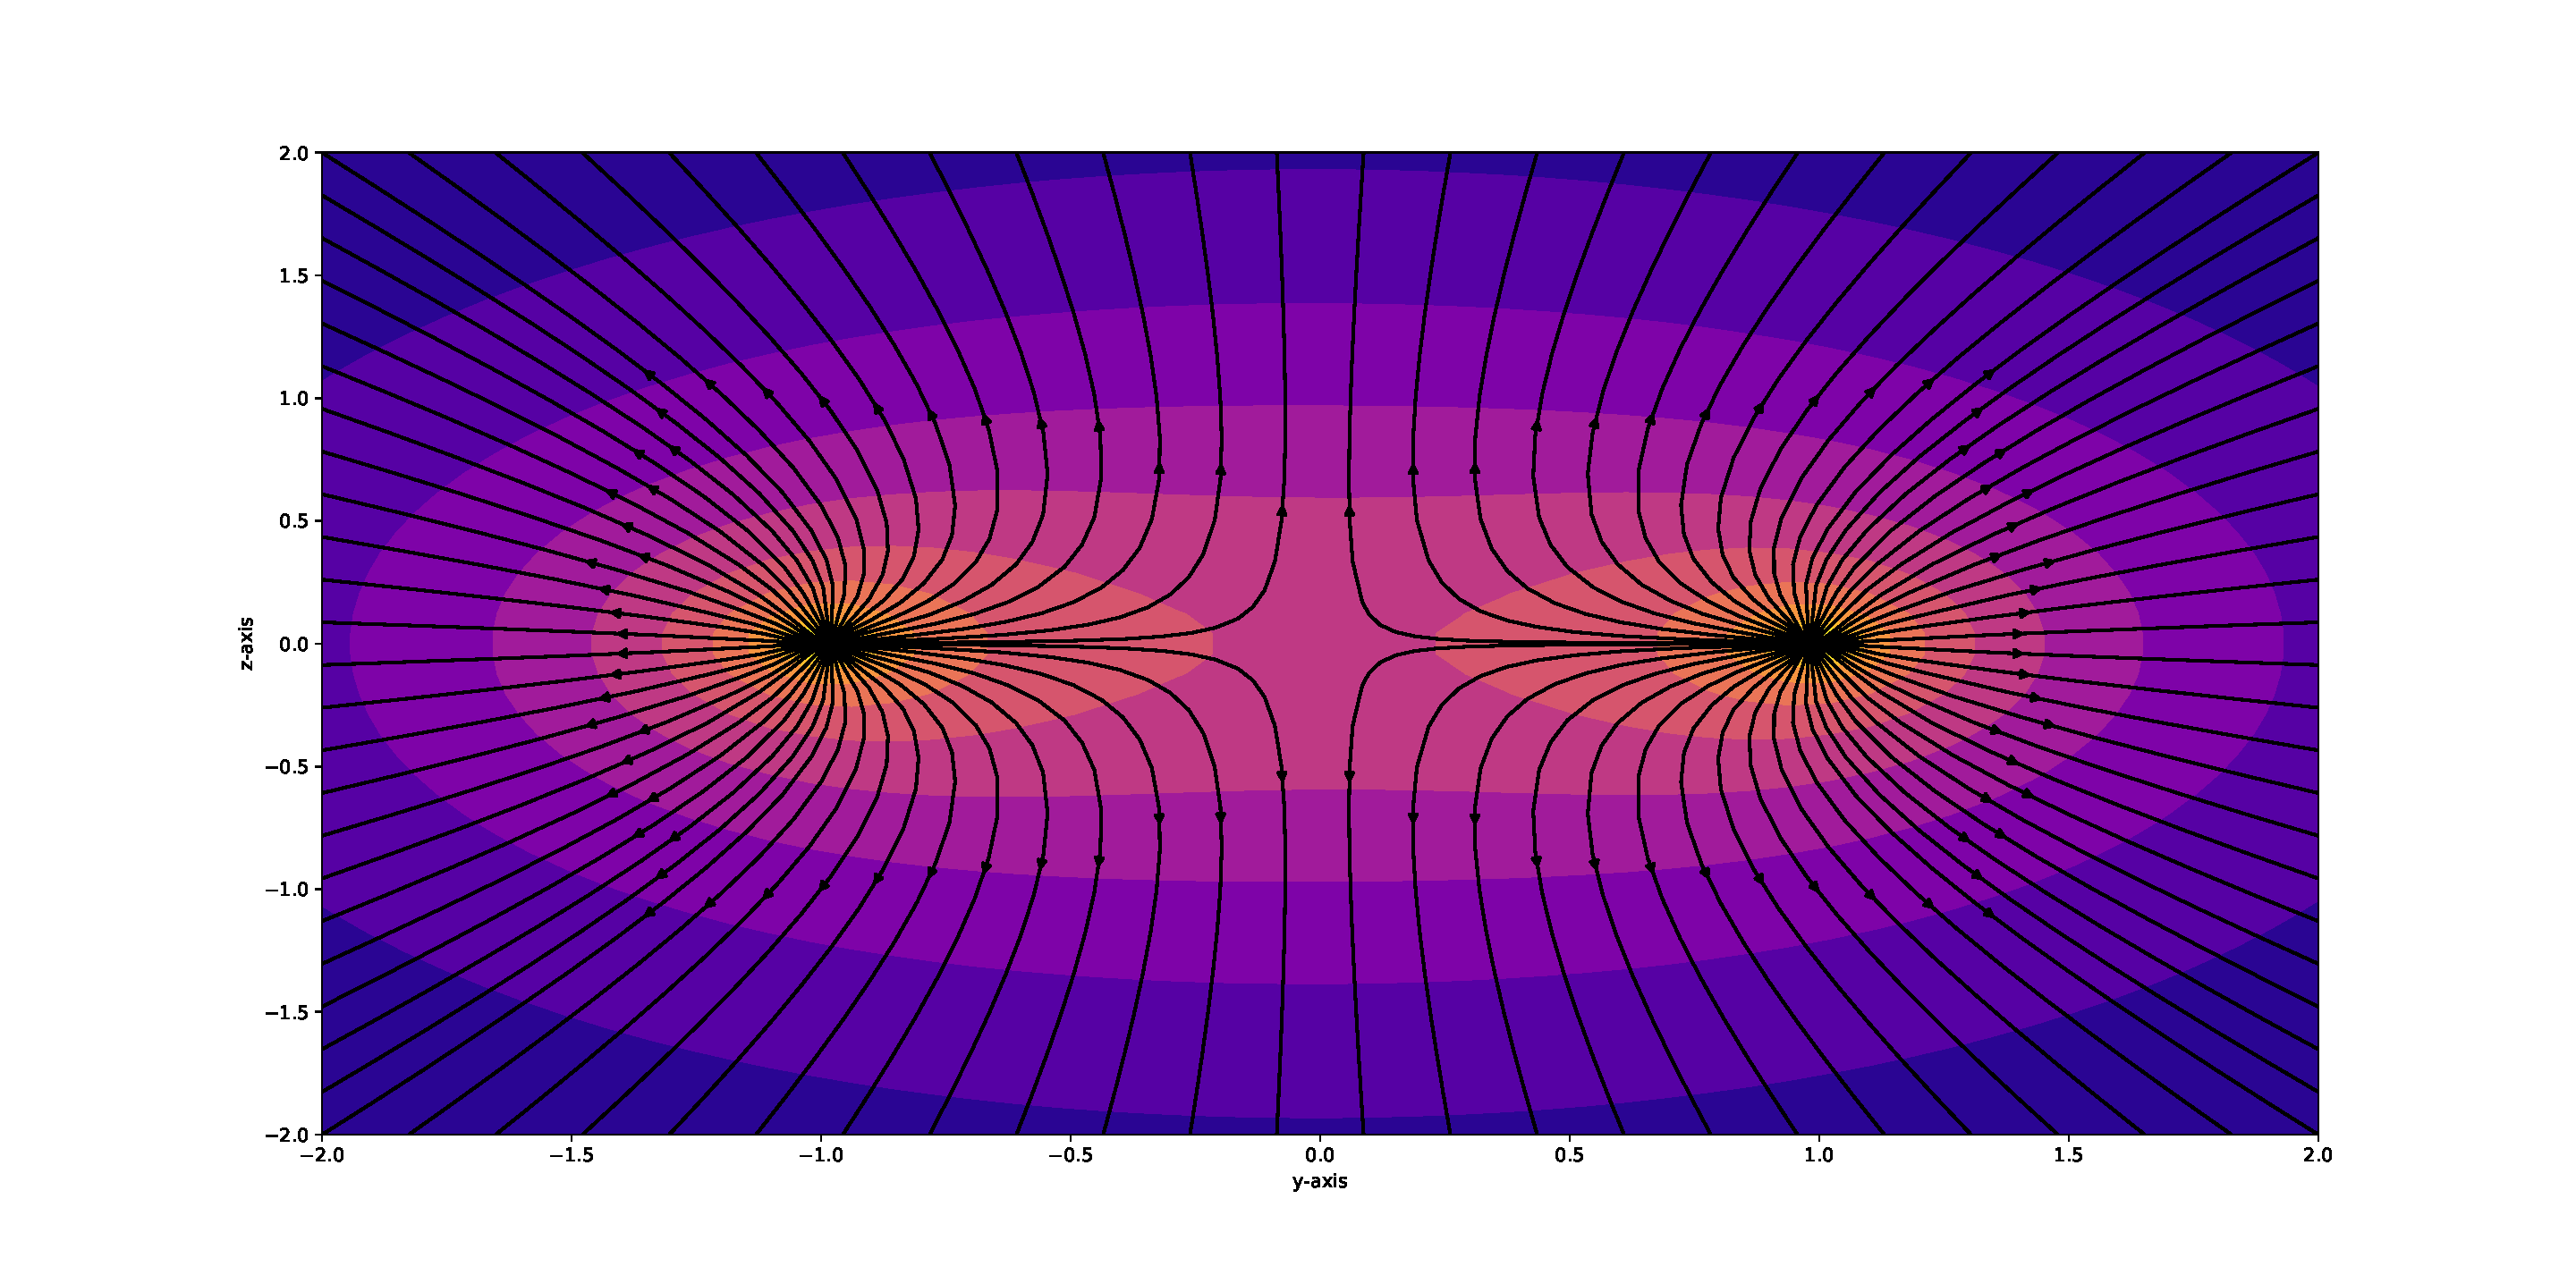
\includegraphics[scale = .3]{Potential_And_Field.pdf}
    \caption{Kontur plot av elektrisk potensialet og strømlinje plot av elektrisk felt}
    \label{fig:figure1}
  \end{figure}  

\section*{d)}
  Planet som ble plottet i forrige oppgave inneholder linjen til z-aksen. Vi kan sammenligne den analytiske løsningen med verdiene fra den midterste søylen i matrisen $ V $. 
  \begin{figure}[h!]
    \centering
    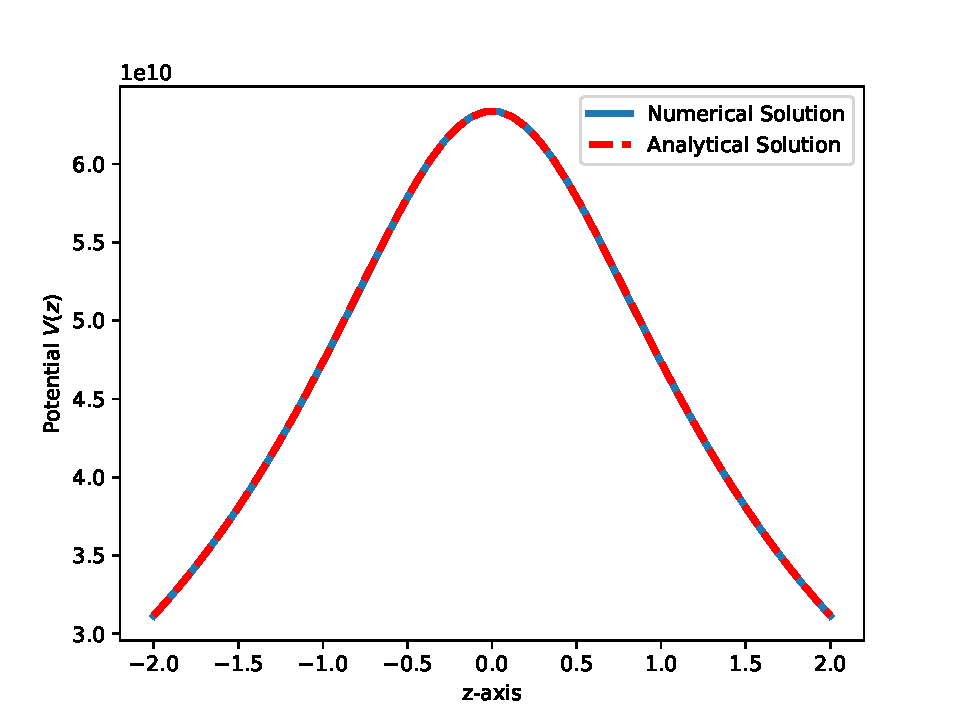
\includegraphics[scale = .45]{Num_vs_Anal.pdf}
    \caption{Numerisk vs Analytisk Løsning }
    \label{fig:figure2}
  \end{figure}

\section*{e)}
  For å finne potensialet fra den øverste firkanten kan vi bruke samme likning som vi fant tidligere \ref{Electric Potential 4lines }, men ladningen endrer fortegn og vi må forskyve z-posisjonen. Da får vi følgende. 
  \begin{equation}\label{Electric Potential 8lines}
    V(z) = - \frac{Q}{4a\piϵ_0}  \operatorname{arcsinh} \left( \frac{a}{\sqrt{a^2 + (2a - z)^2} } \right) 
  \end{equation}
  Legger vi sammen potensialene fra likning \ref{Electric Potential 4lines } \& \ref{Electric Potential 8lines} får vi følgende. 
  \begin{equation}
    V_{tot}(z) = \frac{Q}{4a\piϵ_0} \left( \operatorname{arcsinh} \left( \frac{a}{\sqrt{a^{2}+z^{2}} } \right) - \operatorname{arcsinh} \left( \frac{a}{\sqrt{a^2 + (2a - z)^{2}}}  \right) \right)_{}^{}
  \end{equation}
  Kapasitansen er gitt ved følgende
  \[
  C = \frac{Aϵ_0}{d} = \frac{4a^{2}ϵ_0}{2a}
  \]
  \begin{equation}\label{Kapasitans}
    C = 2aϵ_0
  \end{equation}

\newpage
\section*{Kode}\label{kode_c}
\lstinputlisting[language=python]{FYS-1120_Oblig_1_Kode.py}
\end{document}